\documentclass{assignment}
\ProjectInfos{高等热力学与统计物理}{PHYS2110}{2020-2021学年第二学期}{习题 VI}{截止时间:2021. 4. 13(周二)}{陈稼霖}{45875852}

\begin{document}
\begin{prob}
    计算 Maxwell 分布下的最可几速度,平均速度和速度分布的宽度,即
    \begin{align}
        \Delta v\equiv\sqrt{\langle(v-\langle v\rangle)^2\rangle}
    \end{align}
    将结果用绝对温度和分子质量表达,并算出氢气和氧气以上各量在室温下的数值.
\end{prob}
\begin{sol}
    麦克斯韦速度分布律为
    \begin{align}
        f(v)=\left(\frac{m}{2\pi kT}\right)^{3/2}4\pi v^2e^{-\frac{mv^2}{2kT}}.
    \end{align}
    令上式的导数等于零,
    \begin{align}
        f'(v_0)=\left(\frac{m}{2\pi kT}\right)^{3/2}4\pi v_0e^{-\frac{mv_0^2}{2kT}}\left(2-\frac{mv_0^2}{kT}\right)=0,
    \end{align}
    得最可几速度为
    \begin{align}
        v_0=\sqrt{\frac{2kT}{m}}.
    \end{align}
    平均速度为
    \begin{align}
        \notag\langle v\rangle=&\int_0^{\infty}\mathrm{d}v\,vf(v)=\left(\frac{m}{2\pi kT}\right)^{3/2}4\pi\int_0^{\infty}\mathrm{d}v\,v^3e^{-\frac{mv^2}{2kT}}=\left(\frac{m}{2\pi kT}\right)^{3/2}4\pi\times\frac{2k^2T^2}{m^2}=\sqrt{\frac{8kT}{\pi m}}.
    \end{align}
    速度分布的宽度可表为
    \begin{align}
        \Delta v=\sqrt{\langle v^2\rangle-\langle v\rangle^2},
    \end{align}
    其中速率的平方平均为
    \begin{align}
        \langle v^2\rangle=\int_0^{\infty}\mathrm{d}v\,v^2f(v)=\left(\frac{m}{2\pi kT}\right)^{3/2}4\pi\int_0^{\infty}\mathrm{d}v\,v^4e^{-\frac{mv^2}{2kT}}=\left(\frac{m}{2\pi kT}\right)^{3/2}4\pi\times\frac{3\sqrt{\pi}}{8\left(\frac{m}{2kT}\right)^{5/2}}=\frac{3kT}{m},
    \end{align}
    故速度分布的宽度为
    \begin{align}
        \Delta v=\sqrt{\left(3-\frac{8}{\pi}\right)\frac{kT}{m}}.
    \end{align}
    氢气分子的质量为 $\frac{2\times 10}{6.02\times 10^{23}}$ kg,在室温 $300$ K 下最可几速度为
    \begin{align}
        v_{0,\ce{H2}}=1.58\times 10^3\text{m}\cdot\text{s}^{-1}=1.58\text{km}\cdot\text{s}^{-1},
    \end{align}
    平均速度为
    \begin{align}
        \langle v_{\ce{H2}}\rangle=1.78\times 10^3\text{m}\cdot\text{s}^{-1}=1.78\text{km}\cdot\text{s}^{-1},
    \end{align}
    速度分布的宽度为
    \begin{align}
        \Delta v_{\ce{H2}}=752\text{m}\cdot\text{s}^{-1}.
    \end{align}
    氧气分子的质量为 $\frac{32\times 10^{-3}}{6.02\times 10^{23}}$ kg,在室温下最可几速度为
    \begin{align}
        v_{0,\ce{O2}}=395\text{m}\cdot\text{s}^{-1},
    \end{align}
    平均速度为
    \begin{align}
        \langle v_{\ce{O2}}\rangle=445\text{m}\cdot\text{s}^{-1},
    \end{align}
    速度分布的宽度为
    \begin{align}
        \Delta v_{\ce{O2}}=187\text{m}\cdot\text{s}^{-1}.
    \end{align}
\end{sol}

\begin{prob}
    由同一种分子组成的理想气体被隔膜分成两部分. 每部分的体积,粒子数和温度如右图所示. 假设隔膜左右温度相同,但密度不同,且系统与外界热绝缘. 证明隔膜撤掉后气体的熵增加.
    \begin{figure}[htb]
        \centering
        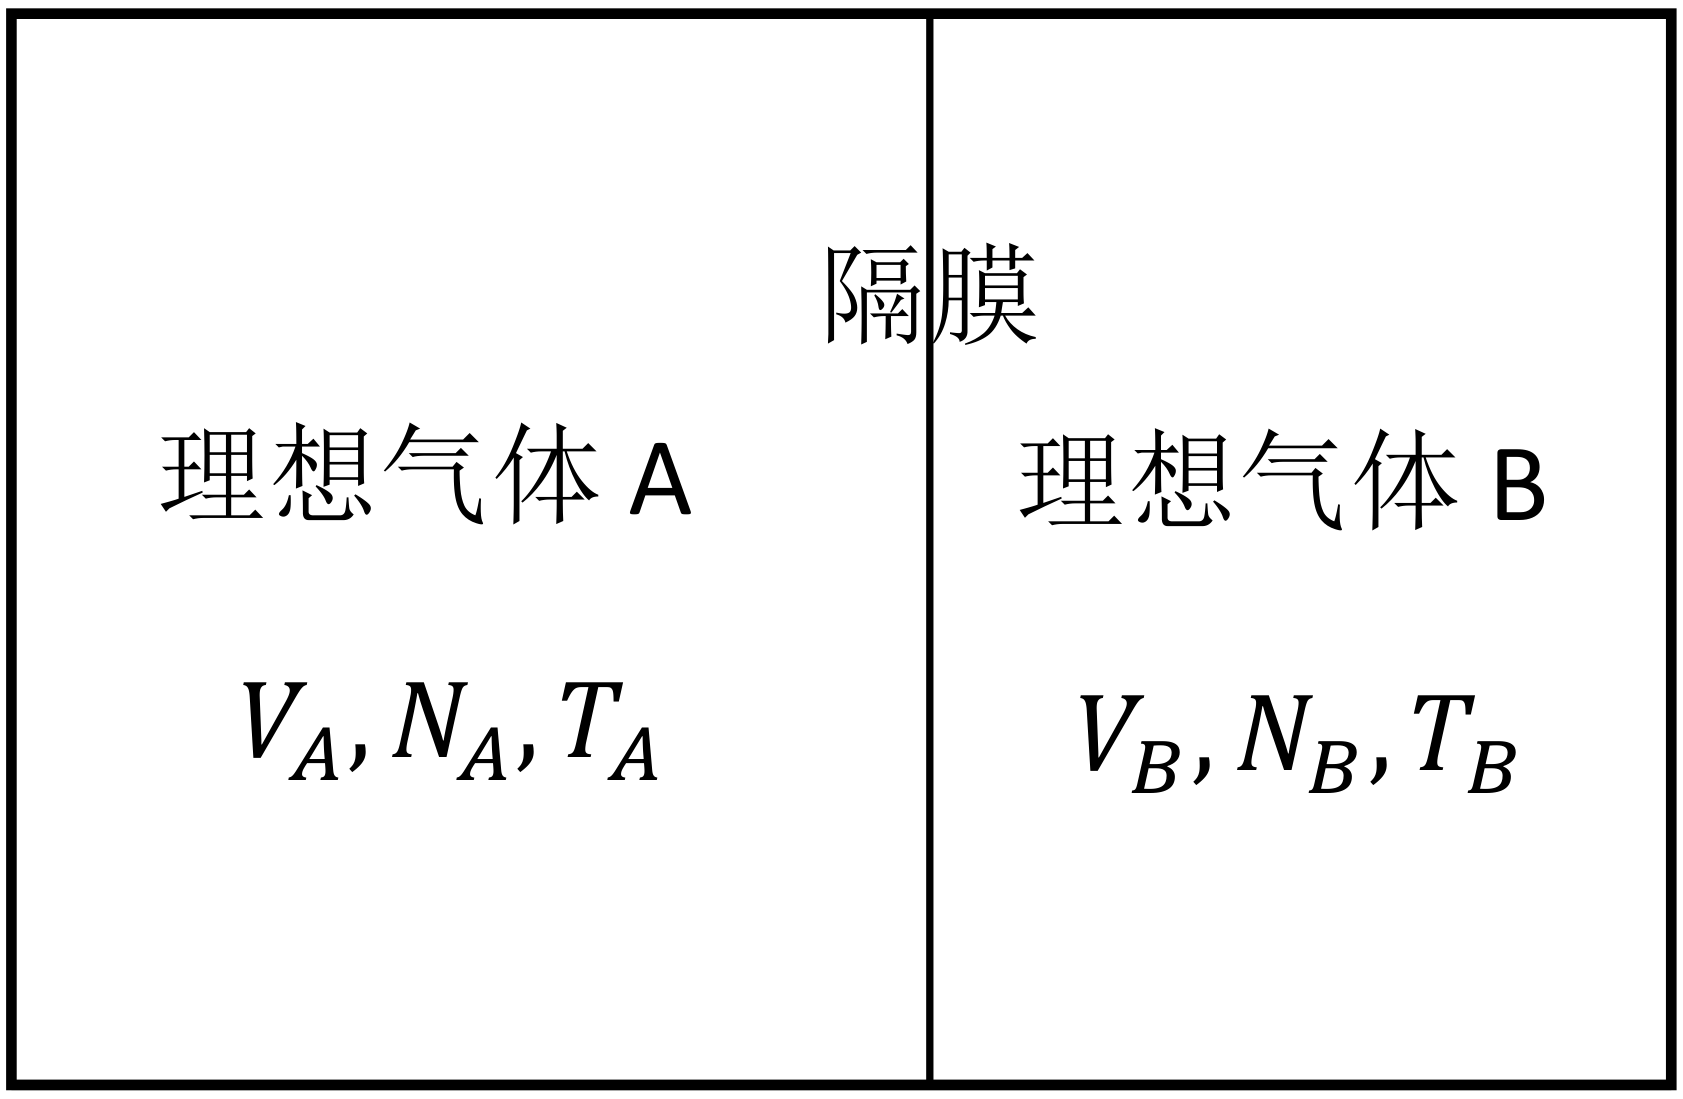
\includegraphics[width=.4\columnwidth]{A6-P2.png}
    \end{figure}
\end{prob}
\begin{pf}
    隔膜撤掉后气体的熵的改变量为
    \begin{align}
        \label{2-DeltaS}
        \notag\Delta S=&S_2-S_1=S_2-S_{1A}-S_{1B}=(N_A+N_B)k\ln\frac{V_A+V_B}{N_A+N_B}-N_Ak\ln\frac{V_A}{N_A}-N_Bk\ln\frac{V_B}{N_B}\\
        =&(N_A+N_B)k\left[\ln\frac{V_A+V_B}{N_A+N_B}-\frac{N_A}{N_A+N_B}\ln\frac{V_A}{N_A}-\frac{N_B}{N_A+N_B}\ln\frac{V_B}{N_B}\right].
    \end{align}
    函数
    \begin{align}
        f(x)=\ln x
    \end{align}
    的二阶导
    \begin{align}
        f''(x)=-\frac{1}{x^2}<0,
    \end{align}
    故 $f(x)$ 为上凸函数. 式 \eqref{2-DeltaS} 中括号内的部分可写作
    \begin{align}
        \notag&\ln\frac{V_A+V_B}{N_A+N_B}-\frac{N_A}{N_A+N_B}\ln\frac{V_A}{N_A}-\frac{N_B}{N_A+N_B}\ln\frac{V_B}{N_B}\\
        =&f\left(\frac{N_A}{N_A+N_B}\frac{V_A}{N_A}+\frac{N_B}{N_A+N_B}\frac{V_B}{N_B}\right)-\frac{N_A}{N_A+N_B}f\left(\frac{V_A}{N_A}\right)-\frac{N_B}{N_A+N_B}f\left(\frac{V_B}{N_B}\right).
    \end{align}
    其中 $\frac{N_A}{N_A+N_B}+\frac{N_B}{N_A+N_B}=1$. 根据上凸函数的性质,
    \begin{gather}
        f\left(\frac{N_A}{N_A+N_B}\frac{V_A}{N_A}+\frac{N_B}{N_A+N_B}\frac{V_B}{N_B}\right)>\frac{N_A}{N_A+N_B}f\left(\frac{V_A}{N_A}\right)+\frac{N_B}{N_A+N_B}f\left(\frac{V_B}{N_B}\right),\\
        \Longrightarrow\ln\frac{V_A+V_B}{N_A+N_B}-\frac{N_A}{N_A+N_B}\ln\frac{V_A}{N_A}-\frac{N_B}{N_A+N_B}\ln\frac{V_B}{N_B}\geq 0.
    \end{gather}
    从而
    \begin{align}
        \Delta S>0,
    \end{align}
    即隔膜撤掉后气体的熵增加.
\end{pf}

\begin{prob}
    在高温条件下,即
    \begin{align}
        \varepsilon\equiv\frac{\hbar^2}{2IkT}\ll 1
    \end{align}
    证明双原子气体的转动配分函数
    \begin{align}
        q_r=\omega\left[\frac{1}{\varepsilon}+\frac{1}{3}+\frac{1}{15}\varepsilon+O(\varepsilon^2)\right]
    \end{align}
    和每个分子平均转动动能
    \begin{align}
        u_r=kT\left[1-\frac{1}{3}\varepsilon-\frac{1}{45}\varepsilon^2+O(\varepsilon^3)\right]
    \end{align}
    其中 $\omega$ 为核自旋的简并度.
    \begin{align}
        \omega=\left\{\begin{array}{ll}
            (2s_A+1)(2s_B+1),&AB\text{型}\\
            \frac{1}{2}(2s_A+1)^2,&AA\text{型}
        \end{array}\right.
    \end{align}
    提示:可用 Euler-Maclaurin 公式计算修正项.
\end{prob}
\begin{pf}
    对于 $AB$ 型双原子分子,转动配分函数为
    \begin{align}
        q_r=(2s_A+1)(2s_B+1)\sum_{j=0}^{\infty}(2j+1)e^{-\varepsilon j(j+1)}.
    \end{align}
    令
    \begin{align}
        f(x)=(2x+1)e^{-\varepsilon x(x+1)},
    \end{align}
    则
    \begin{gather}
        \int_0^{\infty}f(x)\,\mathrm{d}x=\int_0^{\infty}(2x+1)e^{-\varepsilon x(x+1)}\,\mathrm{d}x=\left.-\frac{1}{\varepsilon}e^{-\varepsilon x(x+1)}\right\rvert_0^{\infty}=\frac{1}{\varepsilon},\\
        f(0)=1,\\
        f(\infty)=0,\\
        f^{(1)}(x)=[2-\varepsilon(2x+1)^2]e^{-\varepsilon x(x+1)},\\
        f^{(1)}(0)=2-\varepsilon,\\
        f^{(1)}(\infty)=0,\\
        f^{(3)}(x)=[-\varepsilon^3(2x+1)^4+12\varepsilon^2(2x+1)^2-12\varepsilon]e^{-\varepsilon x(x+1)},\\
        f^{(3)}(0)=-\varepsilon^3+12\varepsilon^2-12\varepsilon,\\
        f^{(3)}(\infty)=0,
    \end{gather}
    利用 Euler-Maclaurin 公式可得
    \begin{align}
        \notag\sum_{j=0}^{\infty}(2j+1)e^{-\varepsilon j(j+1)}=&\int_0^{\infty}f(x)\,\mathrm{d}x+\frac{1}{2}[f(0)-f(\infty)]+(-1)^1\frac{1}{(2\times 1)!}\frac{1}{6}[f^{(1)}(0)-f^{(1)}(\infty)]\\
        \notag&+(-1)^2\frac{1}{(2\times 2)!}\frac{1}{30}[f^{(3)}(0)-f^{(3)}(\infty)]+O(\varepsilon^2)\\
        =&\frac{1}{\varepsilon}+\frac{1}{3}+\frac{1}{15}\varepsilon.
    \end{align}
    从而转动配分函数为
    \begin{align}
        q_r=(2s_A+1)(2s_B+1)\left[\frac{1}{\varepsilon}+\frac{1}{3}+\frac{1}{15}\varepsilon+O(\varepsilon^2)\right].
    \end{align}
    对 $AA$ 型双原子分子,只需将其核自旋的简并度换为 $\frac{1}{2}(2s_A+1)^2$,转动配分函数为
    \begin{align}
        q_r=(2s_A+1)\sum_{j=0}^{\infty}(2j+1)e^{-\varepsilon j(j+1)}=\frac{1}{2}(2s_A+1)\left[\frac{1}{\varepsilon}+\frac{1}{3}+\frac{1}{15}\varepsilon+O(\varepsilon^2)\right].
    \end{align}
    从而一般的转动配分函数可写为
    \begin{align}
        q_r=\omega\left[\frac{1}{\varepsilon}+\frac{1}{3}+\frac{1}{15}\varepsilon+O(\varepsilon^2)\right],
    \end{align}
    其中核自旋简并度
    \begin{align}
        \omega=\left\{\begin{array}{ll}
            (2s_A+1)(2s_B+1),&AB\text{型}\\
            \frac{1}{2}(2s_A+1)^2,&AA\text{型}
        \end{array}\right..
    \end{align}
    每个分子的平均转动动能为
    \begin{align}
        u_r=-\frac{\partial}{\partial\beta}\ln q_r,
    \end{align}
    其中
    \begin{gather}
        \ln q_r=\ln\omega\left[\frac{1}{\varepsilon}+\frac{1}{3}+\frac{1}{15}\varepsilon+O(\varepsilon^2)\right]=\ln\omega-\ln\varepsilon+\ln\left(1+\frac{\varepsilon}{3}+\frac{1}{15}\varepsilon^2+O(\varepsilon^3)\right)=\ln\omega-\ln\varepsilon+\frac{\varepsilon}{3}+\frac{\varepsilon^2}{90}+O(\varepsilon^3),\\
        \frac{\partial}{\partial\beta}\ln q_r=\left[-\frac{1}{\varepsilon}+\frac{1}{3}+\frac{\varepsilon}{45}+O(\varepsilon^2)\right]\frac{\partial\varepsilon}{\partial\beta},\\
        \frac{\partial\varepsilon}{\partial\beta}=\frac{\partial\left(\frac{\hbar^2\beta}{2I}\right)}{\partial\beta}=\frac{\hbar^2}{2I},
    \end{gather}
    故每个分子的平均转动动能为
    \begin{align}
        u_r=\frac{\hbar^2}{2I}\left[\frac{1}{\varepsilon}-\frac{1}{3}-\frac{\varepsilon}{45}+O(\varepsilon^2)\right]=kT\left[1-\frac{\varepsilon}{3}-\frac{\varepsilon^2}{45}+O(\varepsilon^3)\right].
    \end{align}
\end{pf}
\end{document}